\documentclass[a4paper,10pt]{article}
\usepackage[utf8]{inputenc}
\usepackage{graphicx}
\usepackage{array}
\usepackage[center]{caption}

% \usepackage{lmodern}

% \usepackage{concmath}
\usepackage{cmbright}
\usepackage[T1]{fontenc}

\usepackage{amsmath}
\usepackage{amssymb}
\usepackage{mathrsfs}
\usepackage{caption}
\usepackage{array}
\usepackage{lastpage}
% \usepackage[top=3cm, bottom=3cm, left=2cm, right=2cm]{geometry}
\usepackage{tikz}
% \usepackage{epstopdf}

\renewcommand{\labelitemi}{-}

\usepackage{fancyhdr}
\pagestyle{fancy}

\renewcommand{\headrulewidth}{.15pt}
\fancyhead[C]{{Homework Assignment 1}} 
\fancyhead[L]{Page \thepage \ of \pageref{LastPage}}
\fancyhead[R]{MF2007}

\renewcommand{\footrulewidth}{.15pt}
\fancyfoot[C]{\thepage} 
% \fancyfoot[L]{truc}
% \fancyfoot[R]{\leftmark}

\setlength{\columnsep}{1cm}

%opening
\title{MF2007: Dynamic \& Motion Control \\ Homework 1}
\author{Kilian \sc{Demeulemeester}, Jeremy \sc{Pouech}}

\begin{document}

\setlength\parindent{0em}

\maketitle

\section*{Parameter identification} 
\section*{Level 1}



In this section, we need to design the linear friction $d_1$ in the friction model $M_f = d_1 \dot{\varphi}$ and the total inertia $J$.

The parameter identification is done using a step time $T_s = 1 \text{ ms}$.

In order to do so, we add our motor model to the ControlDesk. We then fit the theoretical curves to the real one (using sliders to modify $d_1$ and $J$). 

The fitted curves for motor 1 and motor 2 are on Figure \ref{fittedCurves}.

We get them with the following values:

\begin{center}
\begin{tabular}{|c|c|c|}
 \hline
 & Motor 1 & Motor 2 \\
 \hline 
 $J$ & $4.16e-7$ & $4.16e-7$ \\ 
 \hline 
 $d_1$ & $4.2e-6$ & $4.4e-6$  \\
 \hline
\end{tabular}
\end{center}



\begin{figure}[ht]
%  \includegraphics[width=\Linewidth]{fig/fittedCurvesMotor1.eps}
%  \includegraphics[width=\Linewidth]{fig/fittedCurvesMotor2.eps}
 \caption{Fitted curves for motor 1 \& 2}
 \label{fittedCurves}
\end{figure}




\section*{Level 2}	

\clearpage

\section*{Controlling the motor}

\section*{Velocity control}
\label{velocont}
\addcontentsline{toc}{section}{Velocity control}

\subsection*{Level 1}
\addcontentsline{toc}{subsection}{Level 1}


We need to design a discrete time PI-controller which can be used for the following two reference signals.

\begin{enumerate}
 \item Step response to $300$ rad/s :
 \begin{itemize}
  \item[-] As fast as possible;
  \item[-] No overshoot;
  \item[-] Maximum error at steady state $5$ rad/s.
 \end{itemize}
  \item Sine wave reference signal: \\ $vel_{ref} = 300 \sin(0.2t)$ rad/s.
\end{enumerate}

\begin{center} \noindent\rule{6cm}{0.1pt} \end{center}

In this subsection, $T_s = 1 \text{ ms}$.

In order to design the PI-controller, we use the following method:
\begin{itemize}
 \item Add a continuous PI-controller to the model: $C_{PI}(p) = K(1 + \frac{1}{T_i p})$;
 \item Compute the close loop transfer function of the global system;
 \item Design $K,T_i$ such as there is no overshoot and a fast step response;
 \item Discretize the controller;
 \item Redesign $K,T_i$ in order to fulfill the criteria with the discrete controller.
\end{itemize}

% STEP 1
Let the transfer function for the motor be: $$H_{m}(p) = \frac{K_{m}}{1 + \tau_{m} p}$$

The transfer function for the continuous PI-controller is: $$C_{PI}(p) = K\frac{1 + T_i p}{T_i p}$$

% STEP 2
Thus, the close loop transfer function is: \begin{equation} \label{eq1} H_{cl}(p) = \frac{C_{PI}(p) H_{m}(p)}{1 + C_{PI}(p) H_{m}(p)} \end{equation}

Simplifying equation (\ref{eq1}) leads to: 
\begin{multline} \label{contTransfertPI} H_{cl}(p) = \frac{1 + T_i p}{(1+T_i p)(1+\frac{\tau_{m}}{K K_m} p)} \\ - \frac{1 + T_i p}{(T_i + \frac{\tau_m}{K K_m}p) + (T_i + \frac{T_i}{K K_m}p)} \end{multline}
% \begin{equation} \begin{multline} \label{contTransfertPI} H_{cl}(p) = \frac{1 + T_i p}{(1+T_i p)(1+\frac{\tau_{m}}{K K_m} p) - (T_i + \frac{\tau_m}{K K_m}p) + (T_i + \frac{T_i}{K K_m}p)} \end{multline} \end{equation} 

Let \begin{equation} \label{valueTi} T_i = \tau_m \end{equation}

This value leads to a \emph{first order transfer function in closed loop}.

We then have the following transfer function : \begin{equation} H_{cl}(p) = \frac{1}{1 + \frac{\tau_m}{K K_m}p} \end{equation}

% STEP 3
Let $\tau_{s} = \frac{\tau_m}{K K_m}$ be the new time constant of the system.

\begin{description} \item[Remark :] It seems that the bigger $K$ is, the smaller $\tau_{s}$ is. 
  However, we will see that due to saturation limitation that we can not pick whatever value we want. \end{description}

% STEP 4
The continuous transfer function is discretize using Dustin method $\left(p \leftrightarrow \frac{2}{T_s} \frac{1-z^{-1}}{1 + z^{-1}}\right)$ leads to the following transfer function:

\begin{equation} \label{disTransferPI} \frac{K}{2 T_i} \frac{(2 T_i + T_s) + (T_s - 2 T_i) z^{-1} }{ 1 - z^{-1} } \end{equation}

% STEP 5 
$K$ has to be tuned now. Using Simulink, we create a model of the system including the discrete PI-controller. 

We have the following restriction on $U$ : $U(t) \leq 12 \text{ V}$.

Thus, if $K$ gets too big, the output of the PI-controller is saturated. 

We have the following behavior with K too big:

\begin{center}
\begin{tabular}{c}
  $K$ too big \\ 
  $\downarrow$ \\ The PI-controller output is bigger than $12$ V. \\
  $\downarrow$ \\ $U(t)$ is saturated \\
  $\downarrow$ \\ The PI-controller input error can not decrease \\
  $\downarrow$ \\ The integral part of the controller grows to infinity \\
  $\downarrow$ \\ Once the motor has almost reach its final value, the \\saturation disapear and the big integral part leads\\ to an overshoot
\end{tabular}
\end{center}

In order to avoid these behavior, we use the two following solutions:
\begin{itemize}
 \item K is tuned using an iterative method (the biggest value without any overshoot)
 \item The integral part in the PI-controller is saturated ($|U| \leq 7 \text{ V}$) in order to avoid its growing to infinity in case of a saturation of the output.
\end{itemize}

\emph{This analysis leads to the following understanding : 
Even if our system is modelized by a first order system which can theoreticaly has a step response as fast as we want, 
the saturation in the motor input command leads to response velocity limitations.} \ \newline

This behavior is visible on Figure \ref{stepPIspeed}: for each motor input, the rising velocity is the same. 

Figure \ref{stepPIspeed} and \ref{sinPIspeed} display also that our controller fulfill the criteria for the two reference signals -- with a rise time $t_r \leq 50 \text{ ms}$.

\begin{center}
\begin{figure}[h]
 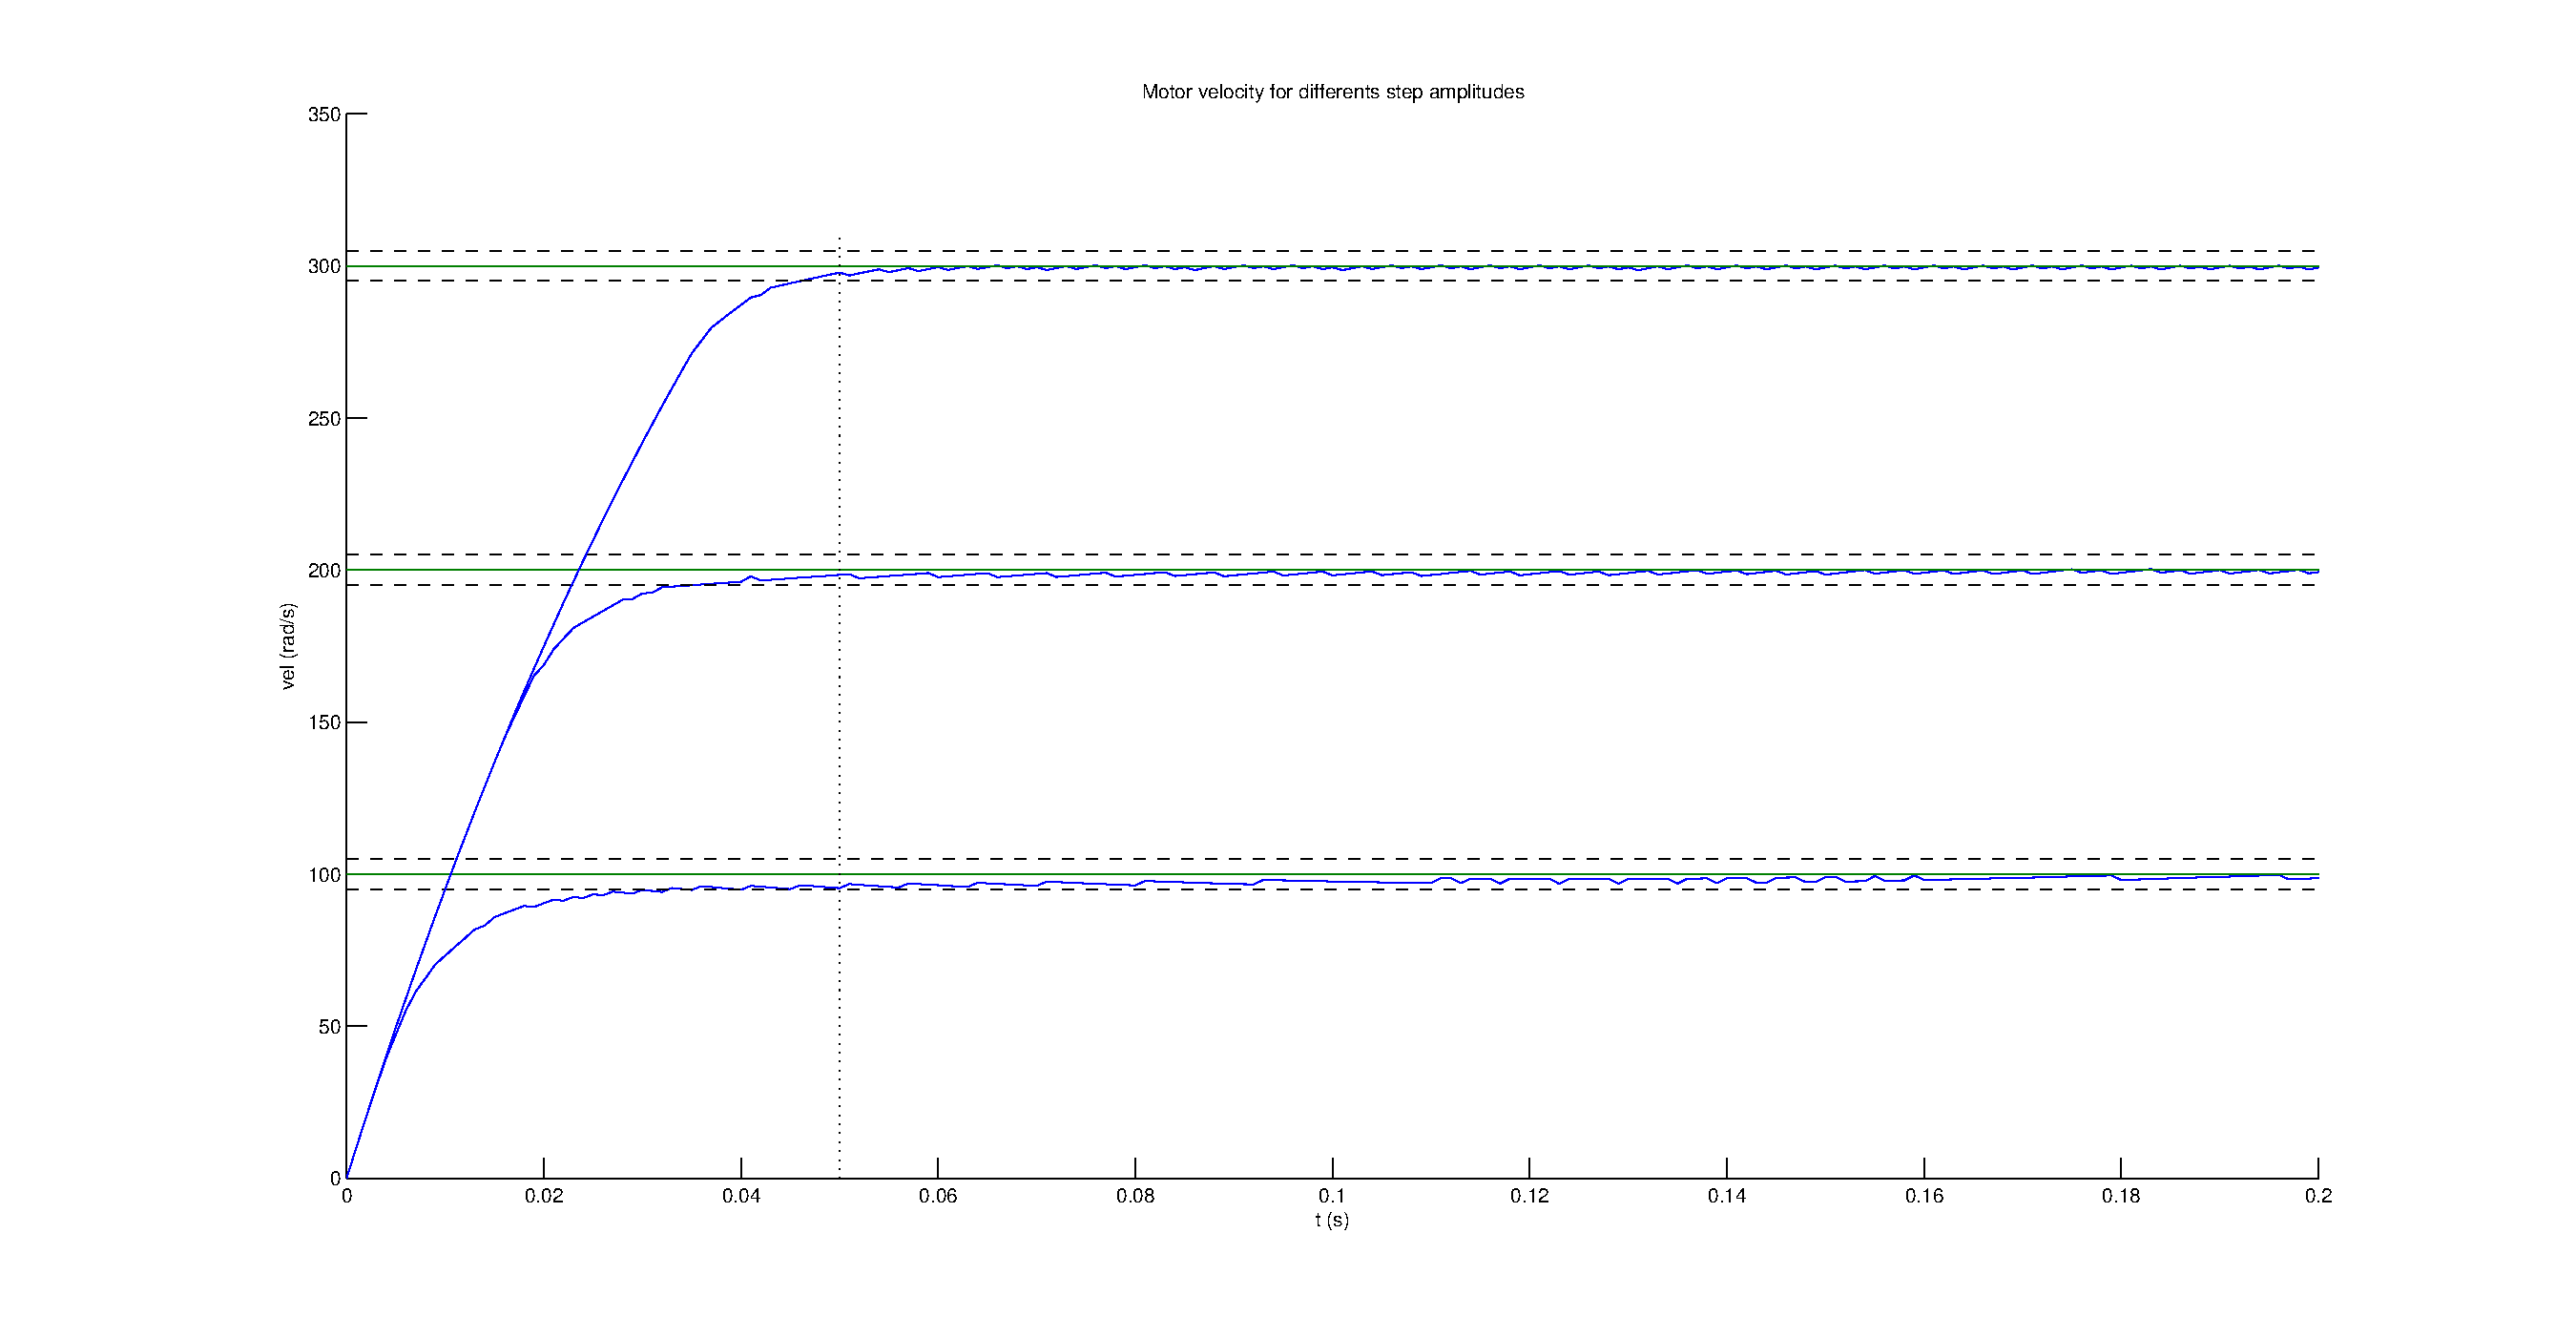
\includegraphics[width=\linewidth]{fig/StepPIspeed.eps}
 \caption{Motor step response for 3 step input of amplitude $(100,200,300)$ rad/s}
 \label{stepPIspeed}
\end{figure}
\end{center}

\begin{center}
\begin{figure}[h]
 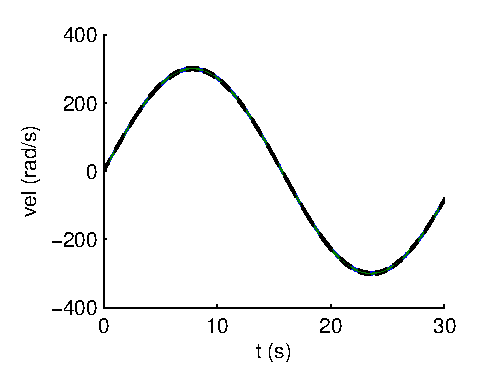
\includegraphics[width=\linewidth]{fig/SinPIspeed.eps}
 \caption{Motor response for the sine wave reference}
 \label{sinPIspeed}
\end{figure}
\end{center}


Using Matlab, we find the following parameters:
\begin{center}
 \begin{tabular}{|c|c|}
 \hline
 $K$ & $T_i$ (s) \\
 \hline
 $0.18$ & $0.8$ \\
 \hline
 \end{tabular}
\end{center}

\clearpage

\section*{Position control}
\addcontentsline{toc}{section}{Position control}

In the two following section, we design a discrete controller that controls the position of the motor, with the following specifications:

\begin{itemize}
 \item Step response to one revolution ($2\pi$) with rise time $t_r = 0.07 \text{ s} \pm 0.005 \text{ s}$.
 \item Maximum overshot $2\%$ of the step ($2\pi$)
 \item Steady state error, maximum $0.5\%$
\end{itemize}


\subsection*{Level 1}


Transforming the temporal criteria of the controller specification to frequency criteria leads to :
\begin{itemize}
 \item Cutoff frequency: $w_c t_r \approx 3 \Leftrightarrow w_c \approx 42.8 \text{ rad/s}$
 \item Phase margin: $D\% \leq 2\% \Leftrightarrow \Delta \Phi \geq 70^{\circ}$ (see Figure \ref{overshootMargin} for this criteria)
\end{itemize}

Moreover, since the position loop include a integrator, the steady state error will be zero.

\begin{center}
\begin{figure}[Ht]
 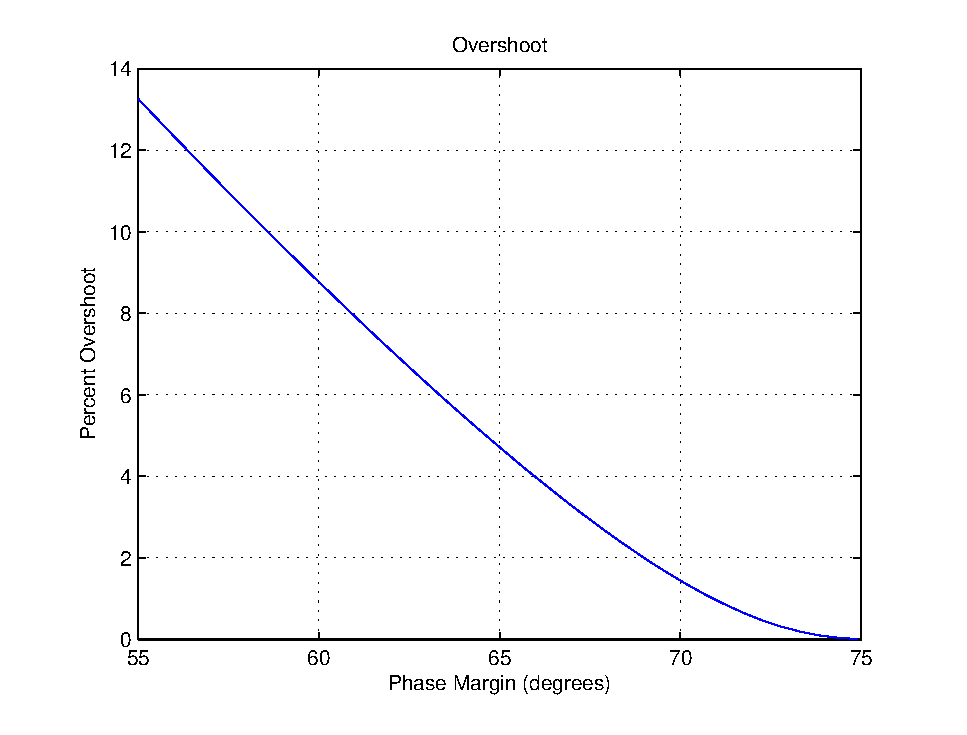
\includegraphics[width=\linewidth]{fig/overshootMargin.eps}
 \caption{Overshoot as a function of the phase margin}
 \label{overshootMargin}
\end{figure}
\end{center}

In this subsection, any sampling period can be used. Here, $T_s = 1 \text{ ms}$.

With the PI-controller from section \ref{velocont}, the ``continuous'' close loop transfer function of the system is:

\begin{equation}
 H_{cl,vel} = \frac{1}{1 + \frac{\tau_m}{K K_m}p}
\end{equation}

Therefore, outputting the position leads to the addition of an integrator block (integration of the velocity). The new transfer function is:

\begin{equation}
 H_{cl,pos} = \frac{1}{p}\frac{1}{1 + \frac{\tau_m}{K K_m}p}
\end{equation}

The maximum rise time for the velocity controller verify $t_{r,vel} \leq 5O \text{ ms} \Leftrightarrow w_c = 125.6 \text{ rad/s}$. Therefore, in the worst case scenario, the transfer function for the position is:

\begin{equation}
 H_{cl,pos} = \frac{1}{p} \frac{1}{1 + \frac{p}{125.6}}
\end{equation}

Figure \ref{bodePos} shows the bode diagram of this function.

\begin{center}
\begin{figure}[Ht]
 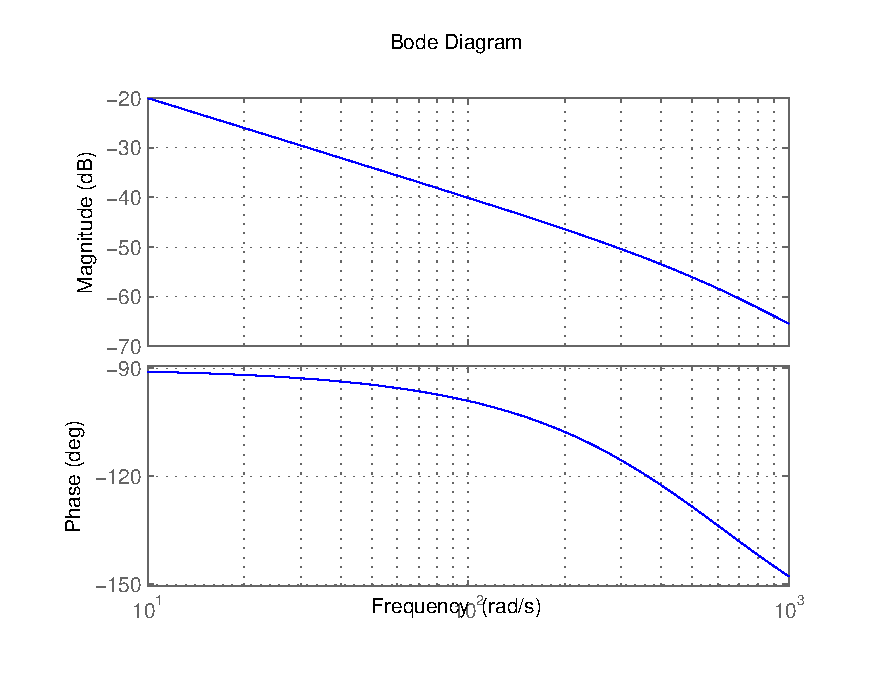
\includegraphics[width=\linewidth]{fig/bodePos.eps}
 \caption{Bode diagram of $H_{cl,pos}$}
 \label{bodePos}
\end{figure}
\end{center}

According to the bode diagram on Figure \ref{bodePos}, we have:

\begin{itemize}
 \item $G_{dB,pos}(\omega = 42.8 \text{ rad/s}) = -32 \text{ dB}$
 \item $\Delta \Phi = 86.3^{\circ}$
\end{itemize}

Therefore, we only need to translate vertically the gain curves in order to fulfill the criteria.

\emph{We use a proportional controller.}

Therefore:

$$ G_{dB,cont}(\omega = 42.8 \text{ rad/s}) = 32 \text{ dB} \Leftrightarrow K_P = 10^{\frac{32}{20}} = 40$$

Figure \ref{StepPPos} shows the step response of the system. \emph{All of the criteria are met.}

\begin{center}
\begin{figure}[Ht]
 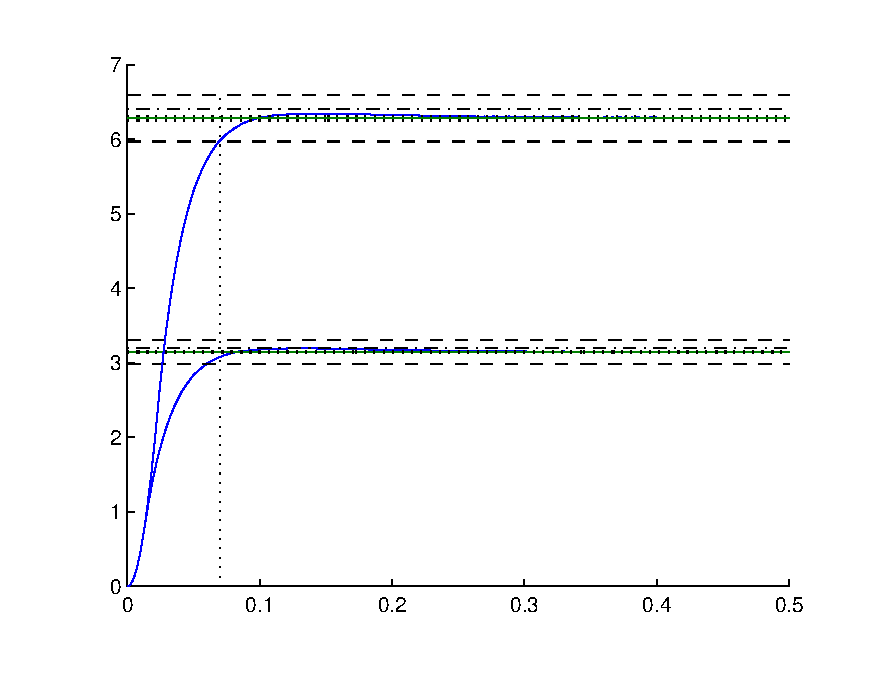
\includegraphics[width=\linewidth]{fig/StepPPos.eps}
 \caption{Steps responses of the system controled in position for two differents amplitudes}
 \label{StepPPos}
\end{figure}
\end{center}









% \clearpage
% 
% \subsection*{Level 2}
\addcontentsline{toc}{subsection}{Level 2}

In this subsection, we want to design the controller with as long as possible sampling period. 

Since we want to fulfill the criteria of $t_r = 0.07 \text{ s} \pm 0.0005 \text{ s}$, the sampling period biggest sampling period is $\frac{t_r}{4} \approx 17 \text{ ms}$.  



\end{document}
